\documentclass[12pt]{article}

\usepackage[margin=1in]{geometry} 
\usepackage{amsmath,amsthm,amssymb}
\usepackage{float}
\usepackage[pdftex]{graphicx}

 

\newcommand{\N}{\mathbb{N}}
\newcommand{\Z}{\mathbb{Z}}

 

\newenvironment{theorem}[2][Theorem]{\begin{trivlist}
\item[\hskip \labelsep {\bfseries #1}\hskip \labelsep {\bfseries #2.}]}{\end{trivlist}}

\newenvironment{lemma}[2][Lemma]{\begin{trivlist}
\item[\hskip \labelsep {\bfseries #1}\hskip \labelsep {\bfseries #2.}]}{\end{trivlist}}

\newenvironment{exercise}[2][Exercise]{\begin{trivlist}
\item[\hskip \labelsep {\bfseries #1}\hskip \labelsep {\bfseries #2.}]}{\end{trivlist}}

\newenvironment{problem}[2][Problem]{\begin{trivlist}
\item[\hskip \labelsep {\bfseries #1}\hskip \labelsep {\bfseries #2.}]}{\end{trivlist}}

\newenvironment{question}[2][Question]{\begin{trivlist}
\item[\hskip \labelsep {\bfseries #1}\hskip \labelsep {\bfseries #2.}]}{\end{trivlist}}

\newenvironment{corollary}[2][Corollary]{\begin{trivlist}
\item[\hskip \labelsep {\bfseries #1}\hskip \labelsep {\bfseries #2.}]}{\end{trivlist}}

 

\begin{document}

 

% --------------------------------------------------------------

%                         Start here

% --------------------------------------------------------------

 

\title{Homework 1}%replace X with the appropriate number
\date{}

 

\maketitle

 

% \begin{theorem}{x.yz} %You can use theorem, exercise, problem, or question here.  Modify x.yz to be whatever number you are proving

% Delete this text and write theorem statement here.

% \end{theorem}

 

% \begin{proof}

% Blah, blah, blah.  Here is an example of the \texttt{align} environment:

% %Note 1: The * tells LaTeX not to number the lines.  If you remove the *, be sure to remove it below, too.

% %Note 2: Inside the align environment, you do not want to use $-signs.  The reason for this is that this is already a math environment. This is why we have to include \text{} around any text inside the align environment.

% \begin{align*}

% \sum_{i=1}^{k+1}i & = \left(\sum_{i=1}^{k}i\right) +(k+1)\\ 

% & = \frac{k(k+1)}{2}+k+1 & (\text{by inductive hypothesis})\\

% & = \frac{k(k+1)+2(k+1)}{2}\\

% & = \frac{(k+1)(k+2)}{2}\\

% & = \frac{(k+1)((k+1)+1)}{2}.

% \end{align*}

% \end{proof}

 

% \begin{theorem}{x.yz}

% Let $n\in \Z$.  Then yada yada.

% \end{theorem}

 

% \begin{proof}

% Blah, blah, blah.  I'm so smart.

% \end{proof}

\begin{problem}{1}
Write in words what each of the following symbols means:
\[
\begin{split}
	\mathrm{(a)}\; &Q \\
	\mathrm{(b)}\; &\overline{MN} \\
	\mathrm{(c)}\; &\vec{ST} \\
	\mathrm{(d)}\; &\overleftrightarrow{FG}
\end{split}
\]
\end{problem}
 
\begin{figure}[H]
\centering
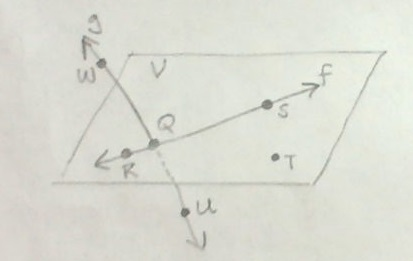
\includegraphics[width=0.5\textwidth]{one.jpg}
\end{figure}

Refer to the figure above for the following problems.

\begin{problem}{2}
Give two other names for $\overleftrightarrow{WQ}$.
\end{problem}

\begin{problem}{3}
Give another name for plane $V$.
\end{problem}

\begin{problem}{4}
Name a point that is not coplanar with $R$, $S$, and $T$.
\end{problem}

\begin{problem}{5}
Is $W$ coplanar with $R$ and $Q$?
\end{problem}

\begin{problem}{6}
What is another name for $\overline{WQ}$?
\end{problem}

\begin{problem}{7}
Name all rays with endpoint $Q$.
\end{problem}

\begin{problem}{8}
Name the intersection of $g$ and $f$.
\end{problem}

\begin{figure}[H]
\centering
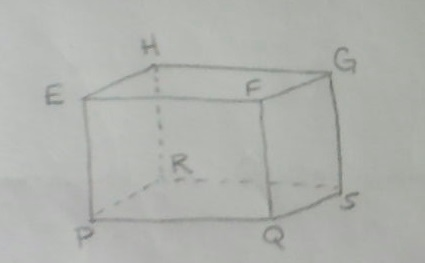
\includegraphics[width=0.5\textwidth]{two.jpg}
\end{figure}
Refer to the figure above for the following problems.

\begin{problem}{9}
Name the intersection of plane $EFG$ and $FGS$.
\end{problem}

\begin{problem}{10}
Why does a four-legged table rock? Does a three-legged table rock?
\end{problem}



\end{document}